\documentclass{article}
%encoding
%--------------------------------------
\usepackage[utf8]{inputenc}
\usepackage[T1]{fontenc}
%--------------------------------------
 
%German-specific commands
%--------------------------------------
\usepackage[ngerman]{babel}
\usepackage{csquotes}
%--------------------------------------

%Pictures
%--------------------------------------
\usepackage{graphicx}
\graphicspath{ {./Pictures/} }
\usepackage{tikz}
\usepackage{subcaption}
\usepackage{float}
\usepackage{wrapfig}
%--------------------------------------

%math
%--------------------------------------
\usepackage{amsmath}
\usepackage{amssymb}
\usepackage{amsfonts}
%--------------------------------------

%Frames
%--------------------------------------
\usepackage{framed}

%Colors
%--------------------------------------
\usepackage{xcolor}
\definecolor{blue-violet}{rgb}{0.54, 0.17, 0.89}
\definecolor{codegreen}{rgb}{0,0.6,0}
\definecolor{codegray}{rgb}{0.5,0.5,0.5}
\definecolor{codepurple}{rgb}{0.58,0,0.82}
\definecolor{backcolour}{rgb}{0.95,0.95,0.92}

%--------------------------------------
\usepackage{multicol}
\usepackage[shortlabels]{enumitem}

%Aufgaben
%--------------------------------------
\usepackage{amsthm}
\newtheorem{aufgabe}{Aufgabe}[section]
\newtheorem{definition}{Definition}[section]
\newtheorem{beispiel}{Beispiel}[section]
\newtheorem*{lernaufgabe*}{Lernaufgabe}
%--------------------------------------

%Listings
%--------------------------------------
\usepackage{ulem}
\usepackage{listings}
 
\lstdefinestyle{mystyle}{
    backgroundcolor=\color{backcolour},   
    commentstyle=\color{codegreen},
    keywordstyle=\color{magenta},
    numberstyle=\tiny\color{codegray},
    stringstyle=\color{codepurple},
    basicstyle=\ttfamily\footnotesize,
    breakatwhitespace=false,         
    breaklines=true,                 
    captionpos=b,                    
    keepspaces=true,                 
    numbers=left,                    
    numbersep=5pt,                  
    showspaces=false,                
    showstringspaces=false,
    showtabs=false,                  
    tabsize=2,
}
 
\lstset{style=mystyle,moredelim=[is][\sout]{|}{|}}
%--------------------------------------


\title{Fliesskommazahlen -- Unterrichtskonzeption}
\author{Alexandra Maximova}
\date{FS2020}

\begin{document}

\maketitle


\section*{Rahmenbedingungen}
Die LPU richtet sich an SuS, die das zweite Semester des Ergänzungsfachs Informatik absolvieren. Die SuS haben Physik und angewandte Mathematik als Schwepunktfach gewählt, und haben keine besondere Mühe mit Mathematik.

Die Fliesskommazahlen sind das zweite Thema im Modul \textbf{'Daten Darstellen'}. In diesem Modul beschäftigen wir uns grundsätzlich mit folgender Frage: Warum sagt man, dass Computer nur Nullen und Einser speichern können, wenn wir doch alle sehen, dass Computer Texte, Bilder und Videos speichern?  Diese haben doch auf dem ersten Blick gar nichts mit Nullen und Einser zu tun.

Das erste Thema des Moduls 'Daten Darstellen' waren ganze Zahlen. Die SuS haben die Zweierkomplement-Darstellung kennengelernt. Das zweite Thema, die Fliesskommazahlen, wurde schon in der vorherigen Stunde eingeführt, und die SuS haben sich schon mit der Kasten-und-Seil Metapher befasst\footnote{Diese Metapher wird genauer unten beschrieben}.

Diese LPU umfasst die zweite und dritte Stunde zum Thema Fliesskommazahlen. In der zweiten Stunde liegt der Fokus auf der Verteilung von den Fliesskommazahlen auf dem Zahlenstrahl und in der dritten Stunde wird die Addition eingeführt.

\section*{Stoffanalyse}
\begin{figure}[H]
\centering
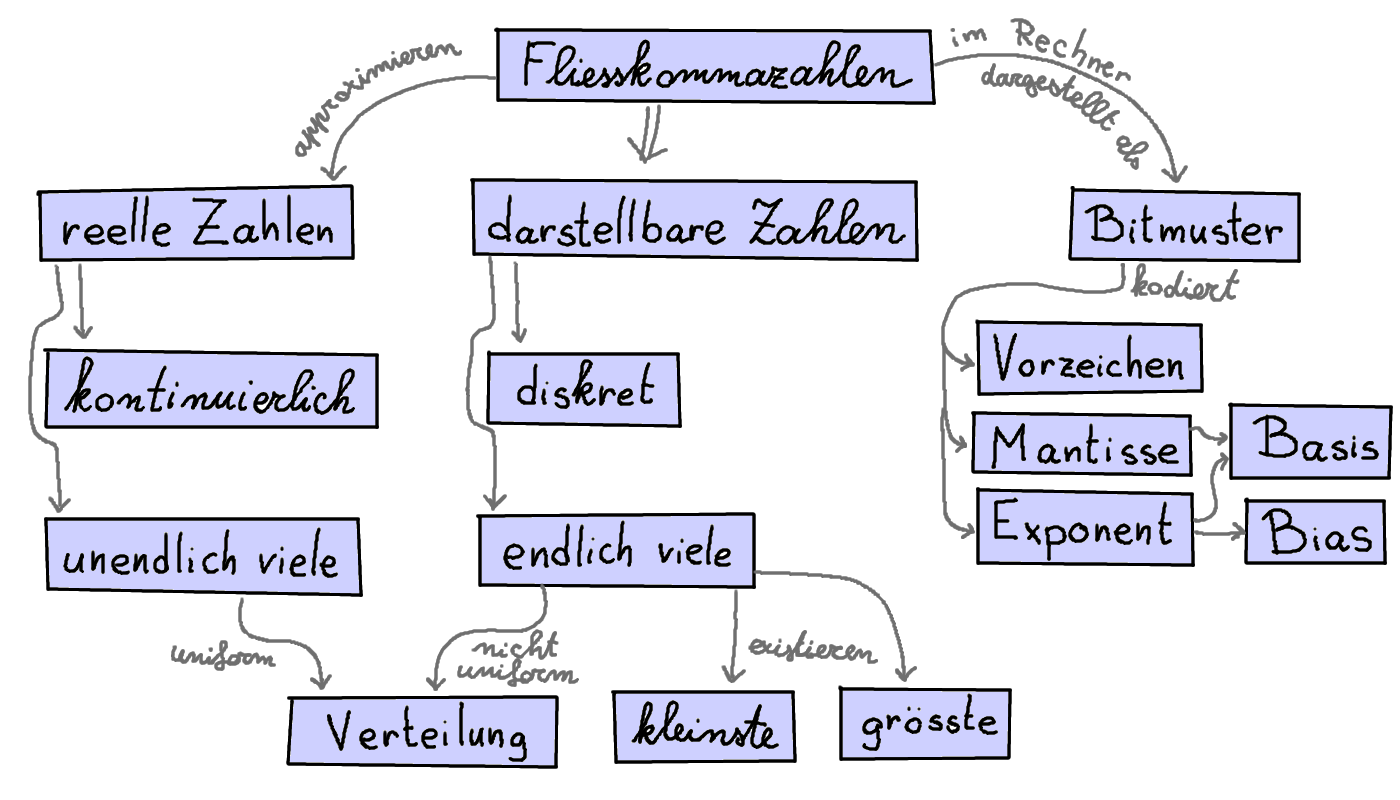
\includegraphics[width=\textwidth]{Pictures/Fliesskommazahlen_Concept_Map.png} 
\end{figure}

Die \textbf{Fliesskommazahlen} werden eingesetzt, um \textbf{reelle Zahlen} zu approximieren. Die reelle Zahlen werden in der Exponentialdarstellung in Basis 2 als \(x = (-1)^s \cdot m \cdot 2^e\) geschrieben, wobei \(s\) das \textbf{Vorzeichenbit} ist, \(m\) die \textbf{Mantisse} und \(e\) der \textbf{Exponent}. Damit die Schreibweise eindeutig ist, verlangt man \(1 \leq m < 10\).

Fliesskommazahlen werden im Computer als \textbf{Bitmuster} kodiert: 1 Bit wird für das Vorzeichenbit \(s\) verwendet, eine fixe Anzahl Bits für die Mantisse \(m\) und eine fixe Anzahl Bits für den Exponenten \(e\). Die Mantisse wird fast eins zu eins übernommen: lediglich das führende ''\(1.\)'' wird weggelassen. Der Exponent, der auch negative Werte einnehmen kann, wird ''zentriert'', indem man zu \(e\) den \textbf{Bias} addiert. Der Bias hängt von der Anzahl Bits ab, die für den Exponenten reserviert sind, und wird meistens so gewählt, dass \(e = 0\) durch die Bitfolge \texttt{100...0} dargestellt wird.

Da im Computer nur eine \textbf{endliche Anzahl Bits} für Mantisse und Exponenten zur Verfügung steht, kann man in einem solchen Zahlensystem nur \textbf{endlich viele} der \textbf{unendlich vielen} reellen Zahlen exakt darstellen. Das bedeutet insbesondere, dass es eine \textbf{kleinste positive darstellbare Zahl}, nämlich \((-1)^0 \cdot 1.000\ldots000 \cdot 2^{e_{min}}\), und eine \textbf{grösste positive darstellbare Zahl}, nämlich \((-1)^0 \cdot 1.111\ldots111 \cdot 2^{e_{max}}\), gibt. Die Exponenten \(e_{min}\) und \(e_{max}\) sind der kleinste, bzw der grösste mögliche Exponent.

Aus der endlichen und fixen Länge von Mantisse und Exponent folgt auch, dass die Fliesskommazahlen \textbf{diskret} sind: Während zwischen zwei reellen Zahlen gibt es immer eine dritte, findet man im Fliesskommazahlensystem Zahlenpaare, zwischen denen keine weitere darstellbare Zahl existiert.

Im Gegensatz zu reellen oder ganzen Zahlen, die auf dem Zahlenstrahl \textbf{gleichmässig verteilt} sind, sind darstellbare Zahlen um die Null konzentriert\footnote{Um ganz exakt zu sein, müsste man aus dieser Beschreibung den Bereich zwischen der grössten negativen darstellbaren Zahl und der kleinsten positiven darstellbaren Zahl ausschliessen} und werden mit wachsendem Exponenten immer zerstreuter.

Die \textbf{Addition} zweier Fliesskommazahlen wird in dieser LPU vereinfacht dargestellt: als erstes bringt man die zwei Zahlen zum gleichen Exponenten, dann addiert man die Mantissen der zwei so enstandenen Zahlen und schliesslich passt man den Exponenten so an, dass für die Mantisse \(m\) gilt: \(1 \leq m < 10\). Das Ergebnis einer solchen Addition könnte mit der Intuition, die wir aus dem Umgang mit rationalen und reellen Zahlen haben, nicht übereinstimmen.


\subsection*{Metapher vom Kasten und Seil}

\begin{figure}[H]
\centering
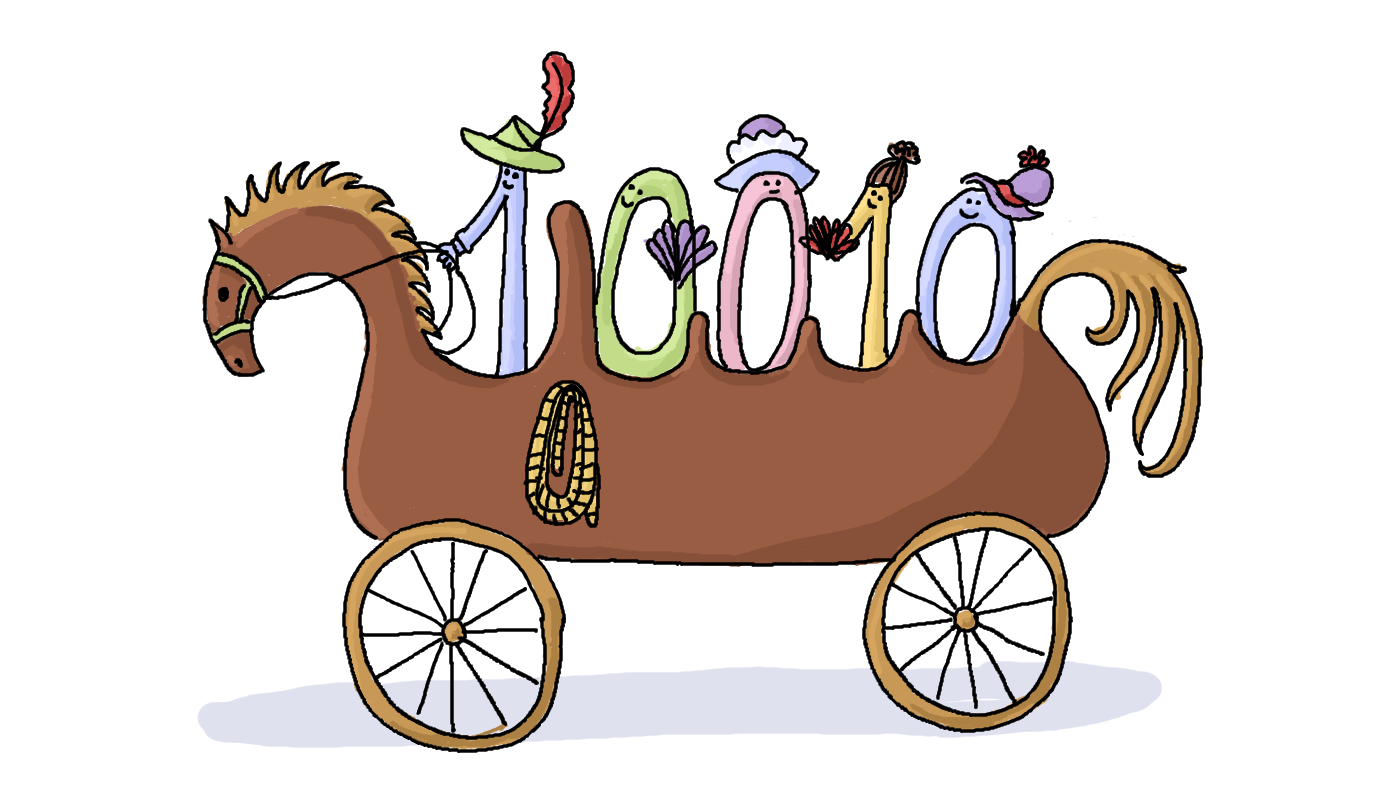
\includegraphics[width=\textwidth]{Pictures/Kutsche.png} 
\end{figure}

Man kann die Endlichkeit und die Bedeutung von Mantisse und Exponent mit einer Metapher illustrieren. Die \textbf{Mantisse} wird mit einem Kasten modelliert, der eine gewisse Anzahl Plätze hat und am Anfang einen speziell markierten Platz, wo nur Einser sitzen können. Der \textbf{Exponent} wir mit einem Seil modelliert. Dieses Seil ist an dem Kasten zwischen der führenden Eins und der nächsten Ziffer fixiert, und zwar so, dass zwei Enden frei sind: das positive Ende nach rechts und das negative Ende nach links. An diesem Seil kann man den Abstand zum ''echten'' Komma markieren. 

Um eine reelle Zahl aus einem solchen Kasten wiederherzustellen, muss man die Markierung am Seil zum ''echten'' Komma anbinden, den Kasten so weit wie möglich ziehen, die leere Plätze bis zum Komma mit Nullen füllen und anschliessend die Ziffern aus dem Kasten aussteigen lassen.

Zu diesem Modell kann man, wenn man will, unterschiedliche Geschichten erzählen:
\begin{description}
\item[Kutsche] Reelle Zahlen werden zum Speicherort mit einer Kutsche transportiert. Diese Kutsche hat nur eine fixe Anzahl Plätze und der Fahrer, der das Pferd manovriert, muss eine Eins sein, weil Nullen keine Händen haben. Damit man weiss, woher man die Ziffern genommen hat, und sie wieder genau dort hinstellen kann, gibt es ein Seil, welcher den Abstand zwischen dem Fahrersitz und dem ''echten'' Komma misst.
\item[Kryobiose] Reelle Zahlen reisen nach Andromeda mit einem Raumschiff. Da die Reise sehr lange dauert und das Raumschiff klein ist, werden die Zahlen in speziellen Eiszellen ''eingefroren'', so dass sie auf Andromeda wieder ''aufgetaut'' werden können. Wie immer, die Eiszellen sind alle gleich und haben Platz nur für eine gewisse Anzahl Ziffern. Zum ''auftauen'' muss man die ''eingefrorene'' Zahlen mit einem speziellen revitalisierendem Kabel an das Komma anschliessen. Die Eiszellen kommen aus der Fabrik mit einer bestimmten Kabellänge, beim ''einfrieren'' darf man den Kabel verkürzen, aber nicht verlängern.
\item[Arche Noah] Reelle Zahlen lesen in der Wettervorhersage, dass bald die nächste Sintflut kommt. Deswegen bestellen sie in der Nachbarfabrik kleine individuellen Archen. Die Archen aus der Fabrik haben eine fixe Anzahl Plätze für die Ziffern und kommen mit einer Kette und einem Anker. Mit Kette und Anker markieren die Zahlen, wie weit die ''geretteten'' Ziffern von dem Komma entfernt sind, so dass, wenn die Sintflut vorbei ist, sie wieder am alten Platz wohnen können.
\end{description}

An diesem Modell sehen die SuS, was passiert, wenn das Seil länger oder kürzer wird, oder der Kasten grösser oder kleiner. Die SuS können experimentieren und sehen, was ist die grösste und was ist die kleinste Zahl, die sie in diesem Modell darstellen können, wie viele Zahlen können sie darstellen und wie weit auseinander benachbarte darstellbare Zahlen sind.

Die Addition kann mit Kasten und Seil auch veranschaulicht werden. Die SuS sehen, warum es keinen Sinn macht, einfach die Mantissen zusammen zu addieren und welche Probleme bei der Addition entstehen können.

\section*{Vorwissen}
\begin{itemize}
\item Die SuS sind mit der Exponentialschreibweise vertraut, z.B. aus der Chemie oder der Physik.
\item Die SuS können ganze Zahlen nach Binär konvertieren.
\item Die SuS haben eine Idee, wie sie rationale Zahlen nach Binär konvertieren könnten: \(i_1 \frac{1}{2} + i_2 \frac{1}{4} + i_3 \frac{1}{8} + \cdots\), wobei die \(i_k\) für Einser oder Nullen stehen. 
\item Die SuS kennen die Zweierkomplement-Darstellung von ganzen Zahlen.
\item Die SuS wissen, wie Fliesskommazahlen im Rechner dargestellt werden:
\begin{itemize}
\item Die SuS wissen, dass der Bitmuster einer Fliesskommazahl aus Vorzeichen, Mantisse und Exponenten besteht.
\item Die SuS kennen die Kasten-und-Seil Metapher.
\end{itemize}
\end{itemize}
Der letzte Punkt ist besonders wichtig und muss gut aktiviert werden.

\section*{Lernziele}

Dieses Thema ist im Modul ''Daten Darstellen'' eingebettet. Die Leitidee vom Modul ist: ''Wenn Computer nur mit Nullen und Einser arbeiten, wie können wir damit rechnen, Texte schreiben, Bilder zeichnen und Videos schneiden?''.

\paragraph{Leitidee} Heutzutage greifen wir zum, möglicherweise im Smartphone integrierten, Taschenrechner beinahe jedes Mal, wenn wir etwas schnell berechnen wollen. Wir glauben, dass der Rechner nicht nur schneller, sondern auch genauer rechnet, als wir Menschen. Das stimmt in den meisten Fällen. Wenn wir aber mit reellen Zahlen zu tun haben, Berechnungen können schnell überraschende Ergebnisse liefern. Damit die SuS nicht unwissend in die Falle der Fliesskommazahlen reinfallen, sollten sie die Struktur und die Besonderheiten der Fliesskommazahlen kennenlernen.

\paragraph{Dispositionsziel} Die SuS vertrauen nicht mehr blind einem Computer bei Berechnungen mit reellen Zahlen.

\paragraph{Operationalisierte Lernziele}
\begin{itemize}
\item Die SuS finden die grösste und kleinste Zahl in einem Fliesskommazahlensystem.
\item Gegeben eine Fliesskommazahl, die SuS schreiben die nächste und die vorherige darstellbare Zahl auf.
\item Die SuS addieren zwei gegebene Fliesskommazahlen.
\end{itemize}




\end{document}
